\documentclass{article}

% 导入宏包
\usepackage{fancyhdr}
\usepackage{ctex}
\usepackage{listings}
\usepackage{graphicx}
\usepackage[a4paper, body={18cm,22cm}]{geometry}
\usepackage{amsmath,amsthm,amssymb,amstext,wasysym,enumerate,graphicx}
\usepackage{float,abstract,booktabs,indentfirst,amsmath}
\usepackage{array}
\usepackage{multirow}
\usepackage{url}
\usepackage{diagbox}
\usepackage{enumitem}
\usepackage{xcolor}
\usepackage{makecell}
\usepackage{tikz}
\usepackage{tcolorbox}
\usetikzlibrary{shapes.geometric, arrows.meta, positioning}
\usepackage[bookmarks=true, colorlinks, citecolor=blue, linkcolor=black]{hyperref}


% 设置段落
\renewcommand\arraystretch{1.4}
\setlength{\parindent}{2em}
\setCJKmonofont{黑体}

% 设置高亮文字
\newtcbox{\mybox}[1][red]
{on line, arc = 0pt, outer arc = 0pt,
	colback = #1!10!white, colframe = #1!50!black,
	boxsep = 0pt, left = 1pt, right = 1pt, top = 2pt, bottom = 2pt,
	boxrule = 0pt, bottomrule = 1pt, toprule = 1pt}

% 配置代码显示
\lstset{
	xleftmargin = 3em,
	xrightmargin = 3em,
	aboveskip = 1em,
	backgroundcolor = \color{white},
	basicstyle = \small\ttfamily,
	rulesepcolor = \color{gray},
	breaklines = true,
	numbers = left,
	numberstyle = \small,
	numbersep = -14pt,
	keywordstyle = \color{purple}\bfseries,
	commentstyle = \color{green!60!black}, % 修改注释颜色
	stringstyle = \color{red!60!green!90!blue!90},
	morekeywords = {ASSERT, int64_t, uint32_t},
	moreemph = {ASSERT, NULL},
	emphstyle = \color{red}\bfseries,
	moreemph = [2]{int64\_t, uint32\_t, tid\_t, uint8\_t, int16\_t, uint16\_t, int32\_t, size\_t, bool},
	emphstyle = [2]\color{purple}\bfseries,
	frame = shadowbox,
	showspaces = false,
	columns = fixed
	morecomment = [l][\color{green!60!black}]{+}, % 设置以+开头的代码行为绿色
}

%--------------------页眉--------------------%

\pagestyle{fancy}
\fancyhead[L]{}
\fancyhead[R]{}
\fancyhead[C]{华东师范大学软件工程学院实验报告}
\fancyfoot[C]{-\thepage-}
\renewcommand{\headrulewidth}{1.5pt}

%--------------------标题--------------------%

\begin{document}
	\begin{center}
		{\Large{\textbf{\heiti 华东师范大学软件工程学院实验报告}}}
		\begin{table}[htb]
			\flushleft
			\begin{tabular}{p{0.4\linewidth}p{0.27\linewidth}p{0.28\linewidth}}\\
				\textbf{实验课程}:数据库系统及其应用实践  & \textbf{年级}:2023级       & \textbf{实验成绩}:  \\
				\textbf{实验名称}:Lab-03 & \textbf{姓名}:顾翌炜         &                 \\
				\textbf{实验编号}:Lab-03     & \textbf{学号}:10235101527 & \textbf{实验日期}:2025/04/03  \\
				\textbf{指导教师}:姚俊杰     & \textbf{组号}:01            & \textbf{实验时间}:2课时  \\ 
			\end{tabular}
		\end{table}
	\end{center}
	\rule{\textwidth}{2pt}
	
	\section{实验目标}
	
	学习和熟悉使用\texttt{SQL}查询处理
	
	参考链接:
	
	https://dev.mysql.com/doc/refman/8.4/en/explain.html
	
	https://dev.mysql.com/doc/refman/8.4/en/explain-output.html
	
	\section{实验要求}
	
	\begin{enumerate}[noitemsep, label={{\arabic*})}]
		\item 按照实验内容,依次完成每个实验步骤;
		
		\item 操作实验步骤时,需要理解该操作步骤的目的,预判操作的结果;当操作结果与预判不符时,及时向任课教师和助教咨询;
		
		\item 在实验报告中依次记录主要操作步骤的内容和结果(返回的消息或截图);
		
		\item 对实验中遇到的问题、解决方案及收获进行总结;
		
		\item 确保实验报告整洁、美观(注意字体、字号、对齐、截图大小和分页等;)
	\end{enumerate}\textbf{}
	
	\section{实验过程记录}
	
	\subsection{环境准备}
	
	首先,连接实验二中的college数据库。我为了后续方便重用,也为了防止源数据被损坏,此处新建了一个\textbf{lab-3\_college}
	
	如下图所示:
	
	\begin{figure}[H]
		\centering
		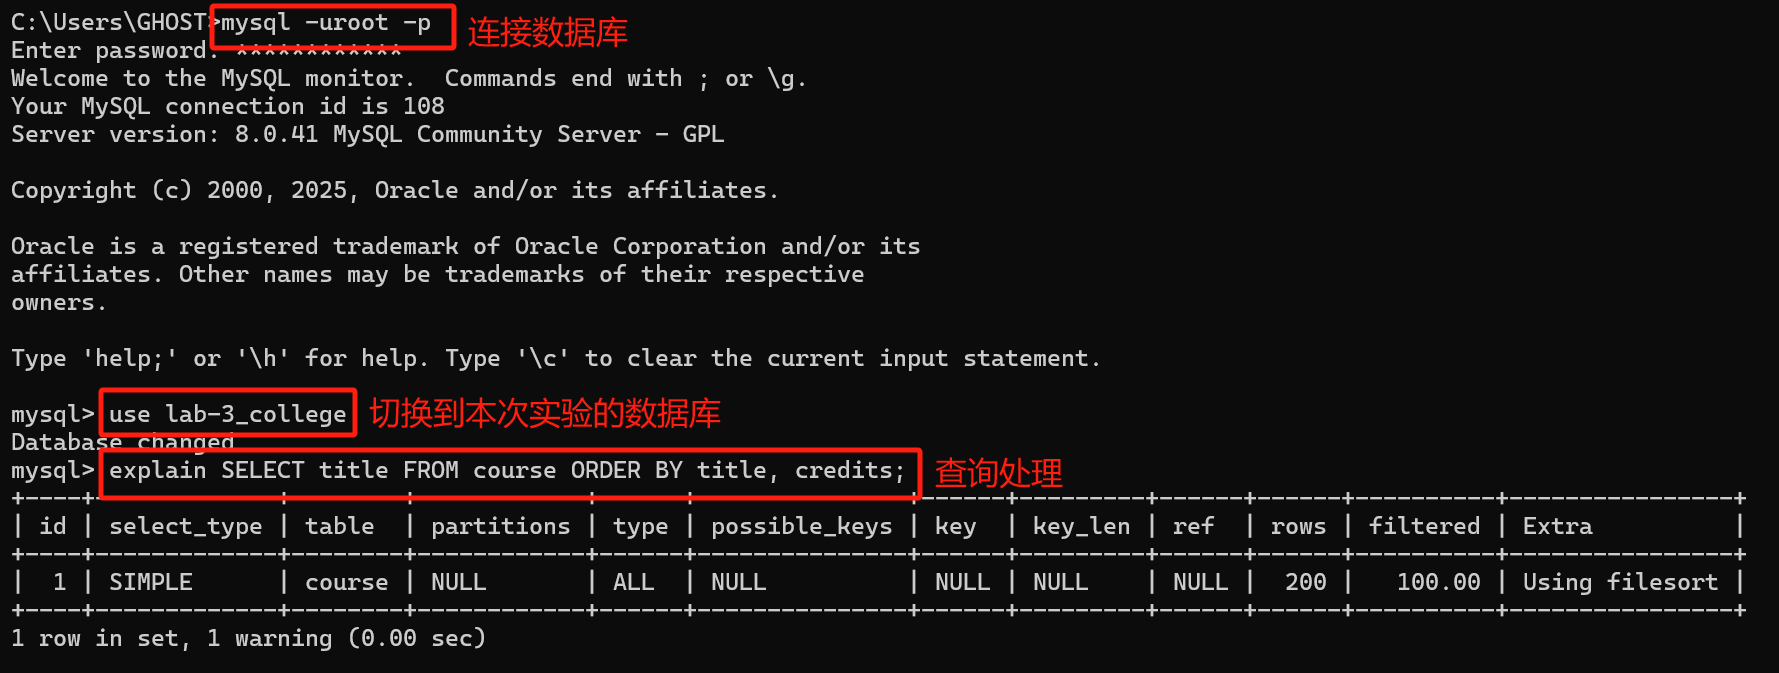
\includegraphics[width=13cm]{./images/1.cmd连接数据库.png}
		\caption{cmd连接数据库}
	\end{figure}
	
	\subsection{EXPLAIN中各个字段的作用与含义}
	
	我们已经通过EXPLAIN语句得到了各个语句的分析,现在需要来通过解释结果来看哪些部分需要进行优化。
	
	通过查阅资料,我们总结为以下表格:
	
	\begin{table}[H]
		\centering
		\begin{tabular}{|l|p{10cm}|}
			\hline
			\textbf{字段名} & \textbf{含义} \\
			\hline
			id & 查询中每个 SELECT 子句的唯一标识符,值越大越先执行 \\
			\hline
			select\_type & SELECT 的类型,如 SIMPLE(简单 SELECT)、PRIMARY(主查询)、SUBQUERY(子查询)等 \\
			\hline
			table & 当前正在访问的表的名称 \\
			\hline
			type & 表的访问方式,性能关键字段(详见下表) \\
			\hline
			possible\_keys & 查询可能使用的索引列表 \\
			\hline
			key & 实际使用的索引,如果为 NULL,说明未使用索引 \\
			\hline
			key\_len & 使用的索引长度(字节数),值越小越高效 \\
			\hline
			ref & 哪一列或常数与 key 一起被使用来选择记录 \\
			\hline
			rows & 估计要读取的行数,越少越好 \\
			\hline
			Extra & 额外信息,如是否使用临时表、排序等 \\
			\hline
		\end{tabular}
		\caption{MySQL EXPLAIN 字段含义}
	\end{table}
	
	其中最重要的是type字段,他决定了这个语句的性能。
	
	这个字段是判断是否需要优化的重要指标,它代表了表的访问方式:
	
	\begin{table}[H]
		\centering
		\begin{tabular}{|l|p{10cm}|}
			\hline
			\textbf{type} & \textbf{含义与性能说明} \\
			\hline
			system & 表仅有一行(系统表),性能最佳 \\
			\hline
			const & 查询结果只匹配一行,通常用于主键或唯一索引查询 \\
			\hline
			eq\_ref & 对于联结中的每一行,从另一个表中读取最多一条匹配记录(使用主键) \\
			\hline
			ref & 使用非唯一索引或前缀索引来查找匹配行 \\
			\hline
			range & 通过索引范围扫描(如 BETWEEN、>、< 等) \\
			\hline
			index & 全索引扫描,不查表,但会扫描整个索引,性能较差 \\
			\hline
			ALL & 全表扫描,最差的访问方式,说明无索引或索引未命中 \\
			\hline
		\end{tabular}
		\caption{MySQL 中 EXPLAIN 的 type 字段含义及性能分析}
	\end{table}
	
	如果我们在返回结果中看到 ALL,说明需要优化。
	
	\subsection{执行计划查询和解释-1}
	
	\begin{lstlisting}[language=sql, title=执行以下语句,获取并解释该查询执行计划, tabsize=4]
		explain SELECT title FROM course ORDER BY title, credits;
		explain analyze SELECT title FROM course ORDER BY title, credits;
	\end{lstlisting}
	
	以上两行运行结果如下图所示:
	
	\begin{figure}[H]
		\centering
		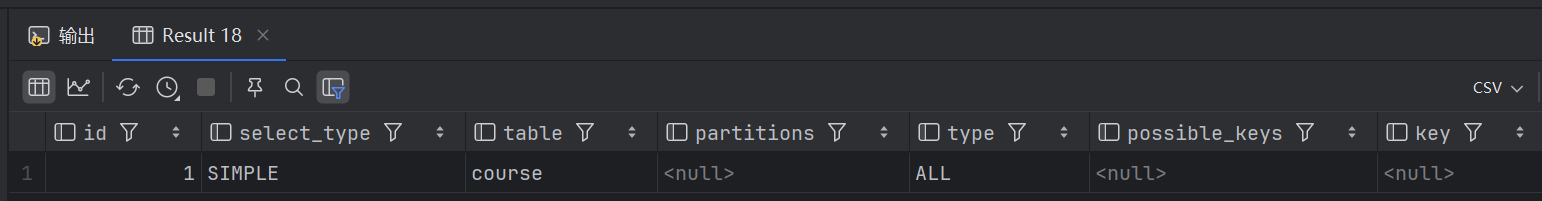
\includegraphics[width=11cm]{./images/2.解释操作1.png}
		\caption{explain操作}
	\end{figure}
	
	\begin{figure}[H]
		\centering
		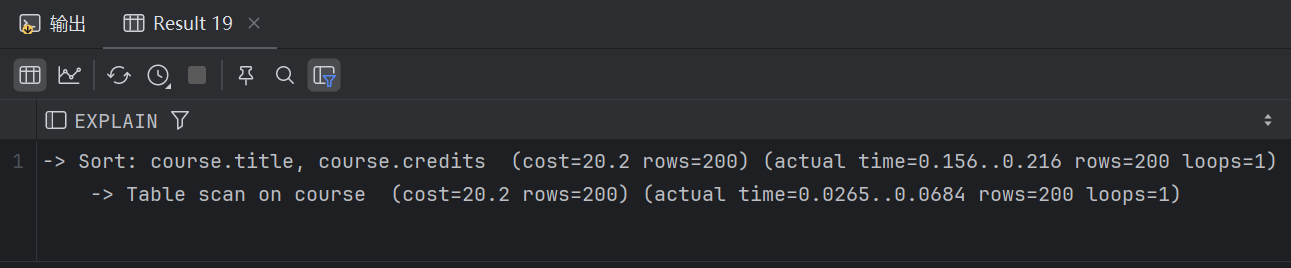
\includegraphics[width=11cm]{./images/3.解释操作2.png}
		\caption{explain analyze操作}
	\end{figure}
	
	执行结果如下图所示:
	
	\begin{table}[H]
		\centering
		\begin{tabular}{|l|l|p{6cm}|l|}
			\hline
			\textbf{字段} & \textbf{含义} & \textbf{结果说明} & \textbf{实际值} \\
			\hline
			\texttt{id} & 查询的执行顺序 & 只有一个简单查询,编号为 1 & 1 \\
			\hline
			\texttt{select\_type} & 查询类型 & \texttt{SIMPLE} 表示没有使用子查询或联合 & SIMPLE \\
			\hline
			\texttt{table} & 涉及的表 & 查询来自 \texttt{course} 表 & course \\
			\hline
			\texttt{type} & 连接类型 & \texttt{ALL} 表示进行了\textbf{全表扫描},是效率最低的一种 & ALL \\
			\hline
			\texttt{possible\_keys} & 可能使用的索引 & 为空,说明没有可用索引 & (null) \\
			\hline
			\texttt{key} & 实际使用的索引 & 也为空,表示没有使用任何索引 & (null) \\
			\hline
			\texttt{key\_len} & 使用索引的长度 & 无索引,因此为 \texttt{(null)} & (null) \\
			\hline
			\texttt{ref} & 哪些列或常数与索引进行比较 & 无引用 & (null) \\
			\hline
			\texttt{rows} & 扫描行数估计 & 预计扫描 200 行(全表) & 200 \\
			\hline
			\texttt{filtered} & 过滤比例估计(百分比) & 预计 100\% 行符合条件 & 100.0 \\
			\hline
			\texttt{Extra} & 附加信息 & \texttt{Using filesort} 表示使用了额外的\textbf{文件排序} & Using filesort \\
			\hline
		\end{tabular}
		\caption{SQL 执行计划详细分析}
	\end{table}
	
	\subsubsection{更清晰的分析结果}
	
	虽然使用 \texttt{EXPLAIN} 能够提供基本的执行计划信息,但在分析复杂查询或调试性能问题时,默认格式可能不够直观。为此,MySQL 提供了更清晰和结构化的格式选项,如 \texttt{FORMAT=TREE} 和 \texttt{FORMAT=JSON},用于展示更详细的执行步骤与优化器决策过程。
	
	\texttt{FORMAT=TREE} 模式以树状结构展示查询的执行流程,使执行顺序和各操作之间的层级关系一目了然,适合人类阅读和理解。而 \texttt{FORMAT=JSON} 模式则输出完整的结构化数据,适合进一步程序处理或自动分析。
	
	对于本实验中的第一条语句:
	
	\begin{lstlisting}[language=sql, title=更清晰和详细的分析结果, tabsize=4]
		explain FORMAT=TREE SELECT title FROM course ORDER BY title, credits;
		explain FORMAT=JSON SELECT title FROM course ORDER BY title, credits;
	\end{lstlisting}
	
	执行上述语句后,得到如下更清晰的分析结果:
	
	\begin{figure}[H]
		\centering
		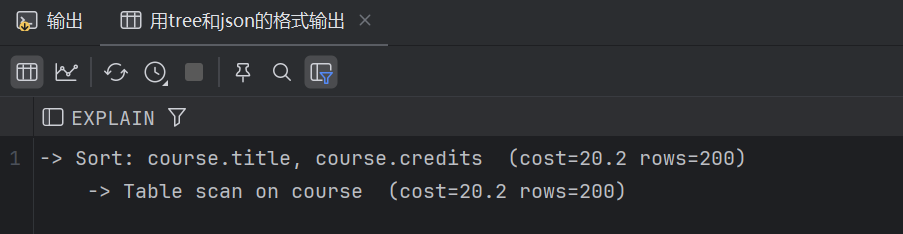
\includegraphics[width=11cm]{./images/4.TREE格式的输出.png}
		\caption{TREE格式的输出}
	\end{figure}
	
	\begin{figure}[H]
		\centering
		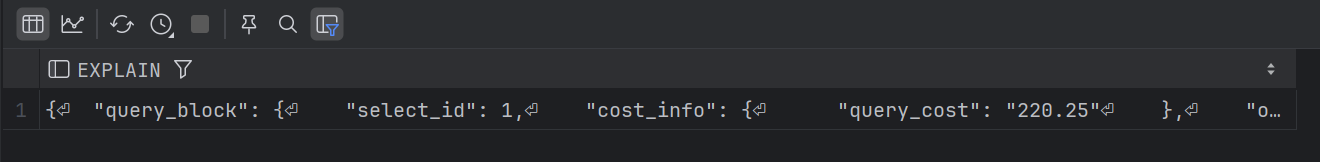
\includegraphics[width=11cm]{./images/5.JSON格式的输出.png}
		\caption{JSON格式的输出}
	\end{figure}
	
	\textbf{进一步分析:}  
	从 \texttt{TREE} 格式的输出中,我们可以直观地看到执行过程为:首先访问 `course` 表的所有行(全表扫描),然后执行排序操作。JSON 格式则显示了更为精细的执行细节,包括优化器选择路径的逻辑判断、排序策略、临时表使用情况等内容。
	
	\textbf{结论:}  
	通过对比不同格式的 EXPLAIN 输出,我们可以更全面地理解查询执行的具体过程,有助于在未来优化更复杂的查询语句时选取合适的手段(如索引、分区、临时表优化等)。
	
	\subsection{执行计划查询和解释-2}
	
	\begin{lstlisting}[language=sql, title=执行以下语句,获取并解释该查询执行计划, tabsize=4]
		explain
		SELECT T1.name
		FROM student AS T1
				JOIN advisor AS T2 ON T1.id = T2.s_id
		GROUP BY T2.s_id
		HAVING count(*) > 1;
		
		explain analyze
		SELECT T1.name
		FROM student AS T1
				JOIN advisor AS T2 ON T1.id = T2.s_id
		GROUP BY T2.s_id
		HAVING count(*) > 1;
	\end{lstlisting}
	
	以上两行运行结果如下图所示:
	
	\begin{figure}[H]
		\centering
		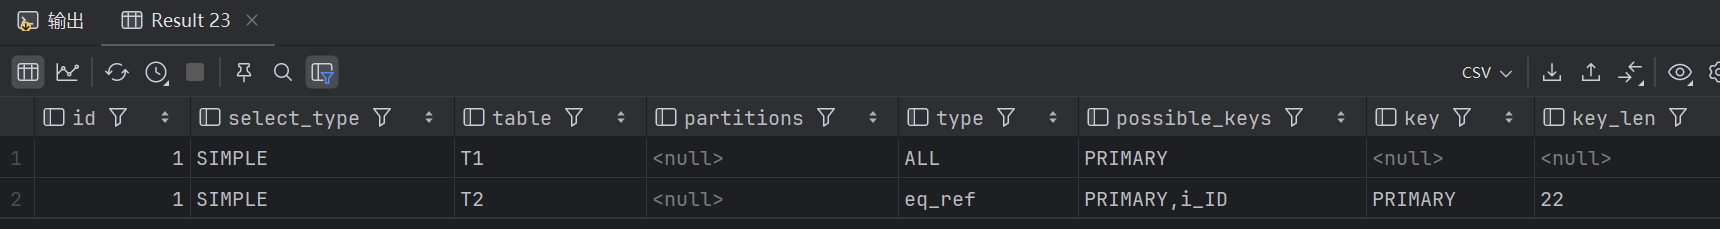
\includegraphics[width=11cm]{./images/6.解释操作1.png}
		\caption{explain操作}
	\end{figure}
	
	\begin{figure}[H]
		\centering
		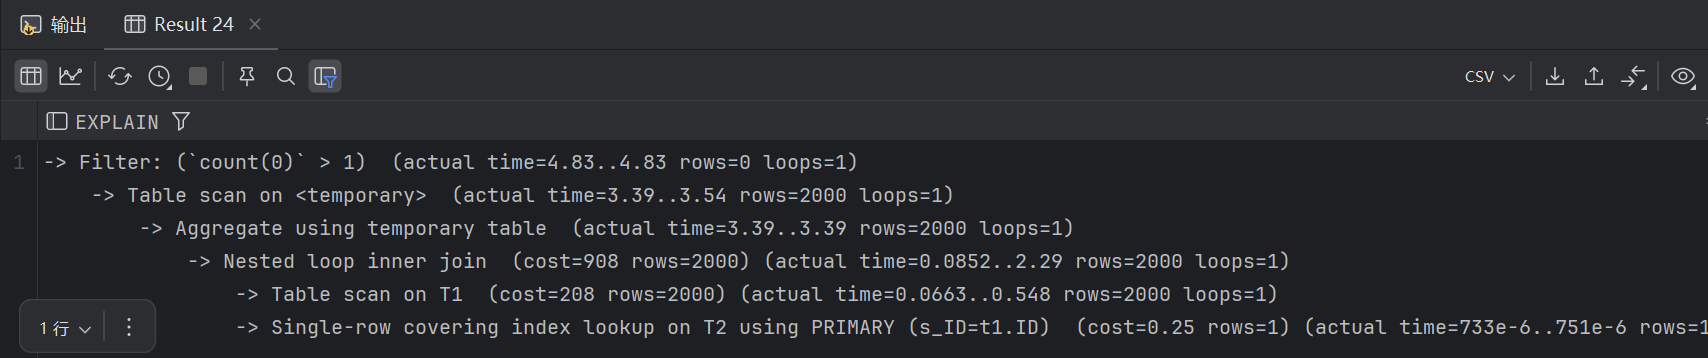
\includegraphics[width=11cm]{./images/7.解释操作2.png}
		\caption{explain analyze操作}
	\end{figure}
	
	我们可以分析得到以下解释信息:
	
	\begin{table}[H]
		\centering
		\begin{tabular}{|l|l|p{4.8cm}|p{4.8cm}|}
			\hline
			\textbf{字段} & \textbf{含义} & \textbf{T1 的值解释} & \textbf{T2 的值解释} \\
			\hline
			\texttt{id} & 查询的执行顺序 & 1,表示第一条执行单元 & 1,表示与 T1 属于同一层查询 \\
			\hline
			\texttt{select\_type} & 查询类型 & SIMPLE,表示基础查询,无子查询 & SIMPLE,亦为基础查询 \\
			\hline
			\texttt{table} & 正在访问的表名 & 表 T1 & 表 T2 \\
			\hline
			\texttt{type} & 连接类型(越靠前效率越低) & ALL,表示对 T1 进行全表扫描 & eq\_ref,表示使用唯一索引连接(效率较高) \\
			\hline
			\texttt{possible\_keys} & 可供选择的索引 & PRIMARY,可用主键索引 & PRIMARY, i\_ID,两个可用索引 \\
			\hline
			\texttt{key} & 实际使用的索引 & 未使用任何索引 & 使用了主键索引 \texttt{PRIMARY} \\
			\hline
			\texttt{key\_len} & 索引长度 & 空值,表示未使用索引 & 22 字节的主键索引长度 \\
			\hline
			\texttt{ref} & 哪些列参与了索引匹配 & 空值,无引用列 & 使用 \texttt{T1.ID} 作为连接条件 \\
			\hline
			\texttt{rows} & 扫描行数估计 & 2000 行(全表扫描) & 1 行(由于主键匹配) \\
			\hline
			\texttt{filtered} & 行过滤比例(百分比) & 100,表示全部行都符合条件 & 100,全部匹配 \\
			\hline
			\texttt{Extra} & 附加信息 & Using temporary,表示使用临时表(可能用于排序或分组) & Using index,表示只访问索引即可返回需要的数据 \\
			\hline
		\end{tabular}
		\caption{T1 与 T2 表连接的执行计划分析}
	\end{table}
	
	\subsection{执行计划查询和解释-3}
	
	\begin{lstlisting}[language=sql, title=执行以下语句,获取并解释该查询执行计划, tabsize=4]
		explain
		SELECT title
		FROM course
		WHERE course_id IN
			(SELECT T1.prereq_id
			 FROM prereq AS T1
					 JOIN course AS T2 ON T1.course_id = T2.course_id
			 WHERE T2.title = 'Mobile Computing');
		
		explain analyze
		SELECT title
		FROM course
		WHERE course_id IN
			(SELECT T1.prereq_id
			 FROM prereq AS T1
					 JOIN course AS T2 ON T1.course_id = T2.course_id
			 WHERE T2.title = 'Mobile Computing');
	\end{lstlisting}
	
	以上两行运行结果如下图所示:
	
	\begin{figure}[H]
		\centering
		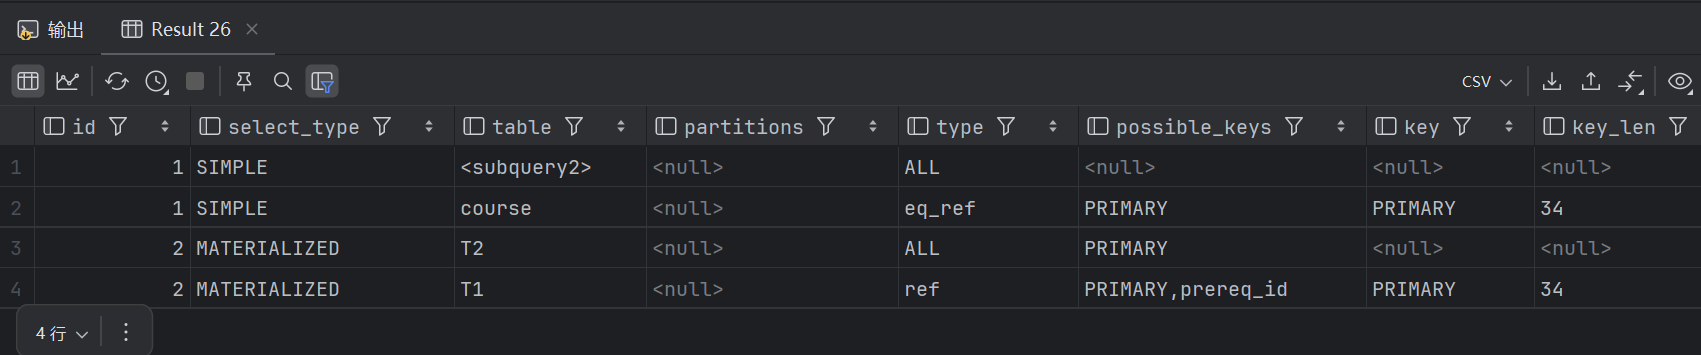
\includegraphics[width=11cm]{./images/8.解释操作1.png}
		\caption{explain操作}
	\end{figure}
	
	\begin{figure}[H]
		\centering
		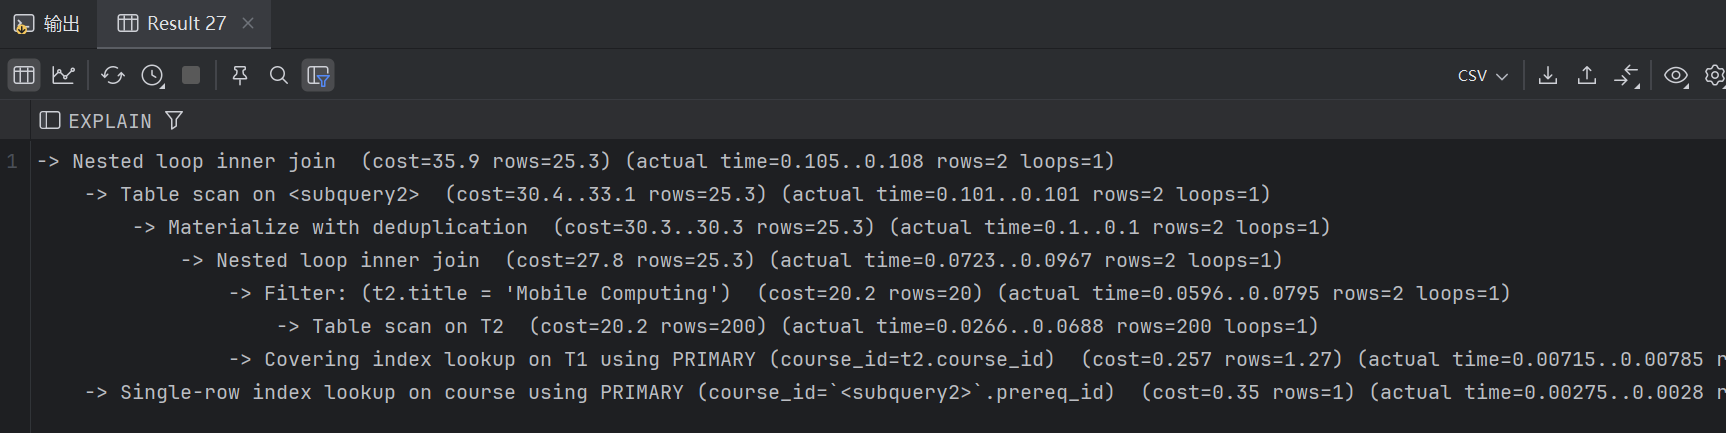
\includegraphics[width=11cm]{./images/9.解释操作2.png}
		\caption{explain analyze操作}
	\end{figure}
	
	我们可以分析得到以下解释信息:
	
	下表展示了对带有 \texttt{IN + 子查询 + JOIN} 的 SQL 语句的执行计划逐项分析:
	
	\begin{table}[H]
		\centering
		\begin{tabular}{|c|l|l|p{9.5cm}|}
			\hline
			\textbf{id} & \textbf{select\_type} & \textbf{table} & \textbf{分析说明} \\
			\hline
			1 & SIMPLE & \texttt{<subquery2>} & 主查询对子查询结果进行 \texttt{IN} 判断。这里的 \texttt{<subquery2>} 是物化后的临时表,使用 \texttt{ALL} 表示全表扫描。表示优化器将子查询缓存为中间结果集,再逐行与 \texttt{course.course\_id} 匹配。 \\
			\hline
			1 & SIMPLE & \texttt{course} & 主查询中的 course 表,通过 \texttt{eq\_ref}(唯一索引等值连接)匹配子查询返回的 prereq\_id,使用主键索引 PRIMARY,性能较好。 \\
			\hline
			2 & MATERIALIZED & \texttt{T2} & 子查询第一部分,对 T2(即 course)做全表扫描(ALL),用于找出 title 为 'Mobile Computing' 的课程。虽然有主键 PRIMARY,但未用到索引筛选条件,可优化。 \\
			\hline
			2 & MATERIALIZED & \texttt{T1} & 子查询第二部分,对 prereq 表通过 ref(索引查找)连接 T2.course\_id,使用了 PRIMARY 和 prereq\_id 的组合索引,性能优良。Extra 中的 \texttt{Using index} 表示只访问了索引。 \\
			\hline
		\end{tabular}
		\caption{四步执行计划分析表}
	\end{table}
	
	\textbf{整体分析:}  \\
	- 子查询首先对 \texttt{T2} 表进行全表扫描(由于缺少 WHERE 子句索引支持),再通过 \texttt{T1.course\_id = T2.course\_id} 做连接;\\
	- 子查询被 MySQL 优化器 \textbf{物化(MATERIALIZED)},即提前执行并缓存结果;\\
	- 主查询使用 \texttt{IN (<subquery2>)} 来过滤符合条件的课程 ID,然后通过主键等值匹配 \texttt{course} 表中的记录;\\
	- \texttt{course} 表通过 \texttt{eq\_ref} 和主键做高效匹配,性能良好;\\
	- 子查询中 \texttt{T1} 表也使用了索引查找,其性能也较好。\\
	
	\subsection{执行计划查询和解释-4}
	
	\begin{lstlisting}[language=sql, title=执行以下语句,获取并解释该查询执行计划, tabsize=4]
		explain
		SELECT dept_name, building
		FROM department
		WHERE budget > (SELECT avg(budget) FROM department);
		
		explain analyze
		SELECT dept_name, building
		FROM department
		WHERE budget > (SELECT avg(budget) FROM department);
	\end{lstlisting}
	
	以上两行运行结果如下图所示:
	
	\begin{figure}[H]
		\centering
		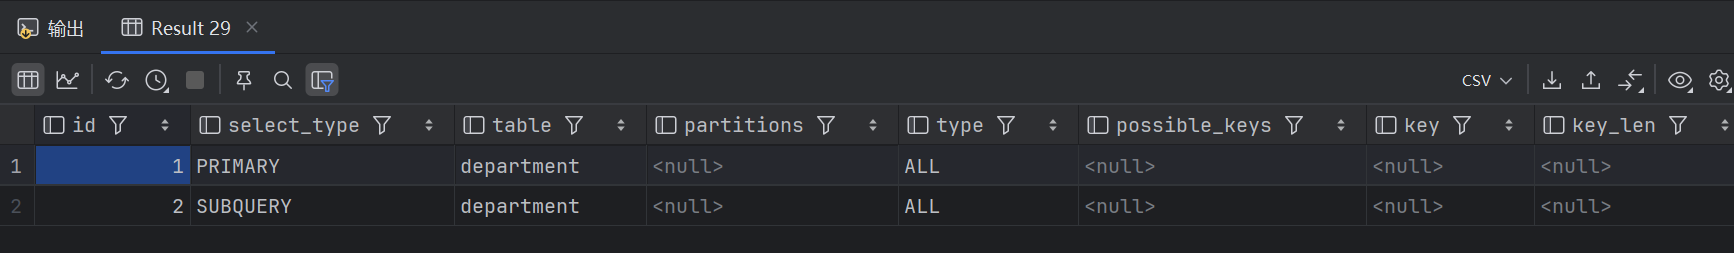
\includegraphics[width=11cm]{./images/10.解释操作1.png}
		\caption{explain操作}
	\end{figure}
	
	\begin{figure}[H]
		\centering
		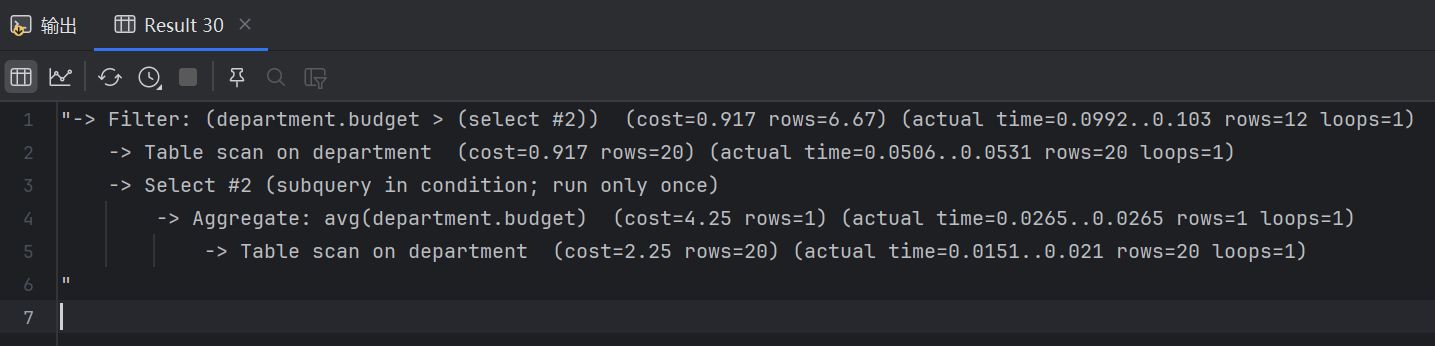
\includegraphics[width=11cm]{./images/11.解释操作2.png}
		\caption{explain analyze操作}
	\end{figure}
	
	我们可以分析得到以下解释信息:
	
	\begin{table}[H]
		\centering
		\begin{tabular}{|l|l|p{4.8cm}|p{4.8cm}|}
			\hline
			\textbf{字段} & \textbf{含义} & \textbf{主查询分析} & \textbf{子查询分析} \\
			\hline
			\texttt{id} & 查询的执行顺序 & 1,表示第一条执行单元(主查询) & 2,表示第二条执行单元(子查询) \\
			\hline
			\texttt{select\_type} & 查询类型 & PRIMARY,表示主查询 & SUBQUERY,表示子查询 \\
			\hline
			\texttt{table} & 正在访问的表名 & department,主查询访问 `department` 表 & department,子查询也访问 `department` 表 \\
			\hline
			\texttt{type} & 连接类型(越靠前效率越低) & ALL,表示全表扫描(效率较低) & ALL,表示全表扫描(效率较低) \\
			\hline
			\texttt{possible\_keys} & 可供选择的索引 & 无,表示没有可用索引 & 无,表示没有可用索引 \\
			\hline
			\texttt{key} & 实际使用的索引 & 无,表示没有使用任何索引 & 无,表示没有使用任何索引 \\
			\hline
			\texttt{key\_len} & 索引长度 & 无,表示未使用索引 & 无,表示未使用索引 \\
			\hline
			\texttt{ref} & 哪些列参与了索引匹配 & 无,表示没有引用列 & 无,表示没有引用列 \\
			\hline
			\texttt{rows} & 扫描行数估计 & 20,预计扫描 20 行数据 & 20,预计扫描 20 行数据 \\
			\hline
		\end{tabular}
		\caption{主查询和子查询的执行计划分析}
	\end{table}
	
	\begin{table}[H]
		\centering
		\begin{tabular}{|l|l|p{4.8cm}|p{4.8cm}|}
			\hline
			\textbf{字段} & \textbf{含义} & \textbf{主查询分析} & \textbf{子查询分析} \\
			\hline
			\texttt{filtered} & 行过滤比例(百分比) & 33.33,表示大约 33.33\% 的行符合主查询条件 & 100,表示子查询返回了所有符合条件的行 \\
			\hline
			\texttt{Extra} & 附加信息 & Using where,表示主查询使用了 `WHERE` 子句过滤数据 & 无,子查询没有额外信息 \\
			\hline
		\end{tabular}
		\caption{主查询和子查询的执行计划分析-续}
	\end{table}
	
	\subsection{项目查询分析}
	
	对实验2中的小项目作业中涉及的SQL查询语句,使用 \texttt{EXPLAIN} 语句进行分析:
	
	\begin{enumerate}
		\item 画出查询计划树,说明每个节点的功能和执行时间信息。
		\item 说明该执行计划是否为最优的。
		\item 针对可能出现的性能问题,提出解决方案。(若为最优的,尝试做一个较差的执行方案并说明性能差距出现的原因。)
	\end{enumerate}
	
	\subsubsection{提取Lab-2中使用到的sql语句}
	
	首先从Lab-2的JDBC代码中提取出主要的sql语句:
	
	\begin{tcolorbox}[title = {备注}, colback = blue!25!white, colframe = blue!75!black]
		JDBC中使用了?来预留参数的位置,此处为了检验查询,我们使用id=1000的这位同学来进行实验
	\end{tcolorbox}
	
	主要包括了:
	
	\begin{lstlisting}[language=sql, title=Lab-2中的sql语句, tabsize=4]
		SELECT ID, name, dept_name, tot_cred
		FROM student
		WHERE name LIKE 'man';
		
		SELECT ID, name, dept_name, tot_cred
		FROM student
		WHERE ID = 1000;
		
		SELECT takes.course_id, year, semester, title, dept_name, grade, credits
		FROM takes
				JOIN course ON takes.course_id = course.course_id
		WHERE ID = 1000;
		
		SELECT grade_point, credits
		FROM (takes JOIN course ON takes.course_id = course.course_id)
				JOIN gpa ON gpa.grade = TRIM(takes.grade)
		WHERE ID = 1000;
	\end{lstlisting}
	
	\subsubsection{EXPLAIN ANALYZE Lab-2中的语句}
	
	\begin{lstlisting}[language=sql, title=EXPLAIN ANALYZE Lab-2中的语句, tabsize=4]
		EXPLAIN
		SELECT ID, name, dept_name, tot_cred
		FROM student
		WHERE name LIKE 'man';
		
		EXPLAIN
		SELECT ID, name, dept_name, tot_cred
		FROM student
		WHERE ID = 1000;
		
		EXPLAIN
		SELECT takes.course_id, year, semester, title, dept_name, grade, credits
		FROM takes
				JOIN course ON takes.course_id = course.course_id
		WHERE ID = 1000;
		
		EXPLAIN
		SELECT grade_point, credits
		FROM (takes JOIN course ON takes.course_id = course.course_id)
				JOIN gpa ON gpa.grade = TRIM(takes.grade)
		WHERE ID = 1000;
	\end{lstlisting}
	
	得到的结果如下图所示:
	
	\begin{figure}[H]
		\centering
		\begin{minipage}[b]{0.45\textwidth}
			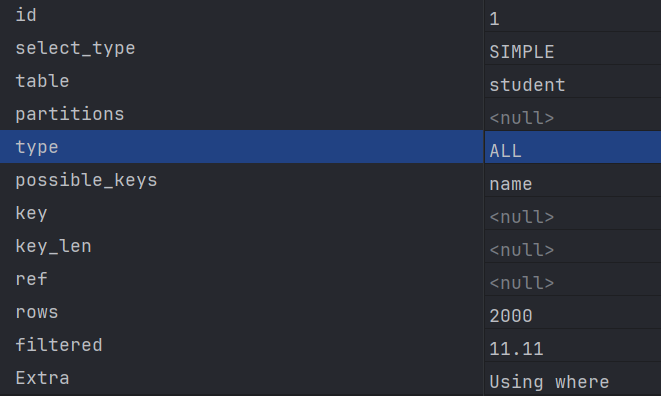
\includegraphics[width=\textwidth]{./images/12.EXPLAIN-1.png}
			\caption{第一个语句的EXPLAIN结果}
		\end{minipage}
		\hfill
		\begin{minipage}[b]{0.45\textwidth}
			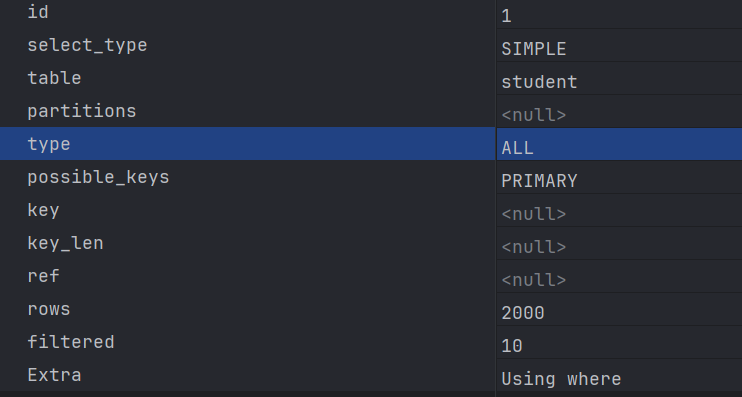
\includegraphics[width=\textwidth]{./images/13.EXPLAIN-2.png}
			\caption{第二个语句的EXPLAIN结果}
		\end{minipage}
	\end{figure}
	
	\begin{figure}[H]
		\centering
		\begin{minipage}[b]{0.45\textwidth}
			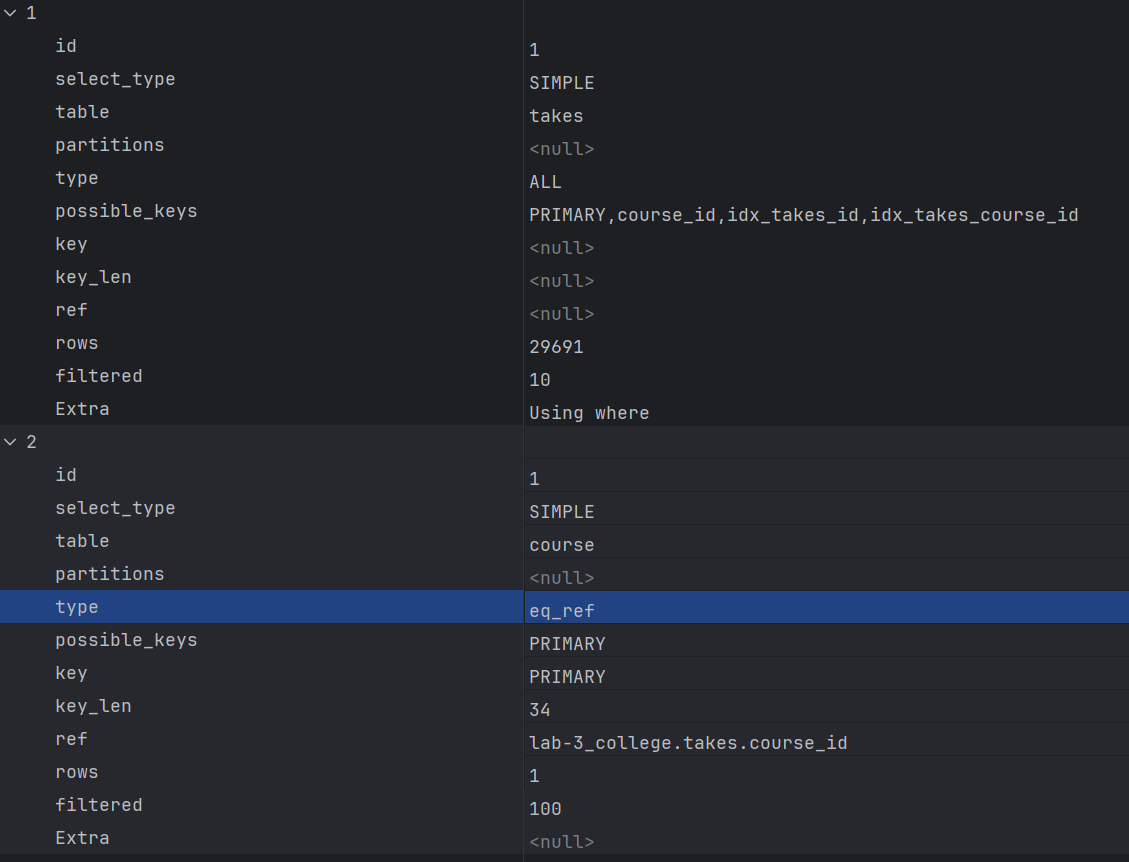
\includegraphics[width=\textwidth]{./images/14.EXPLAIN-3.png}
			\caption{第三个语句的EXPLAIN结果}
		\end{minipage}
		\hfill
		\begin{minipage}[b]{0.45\textwidth}
			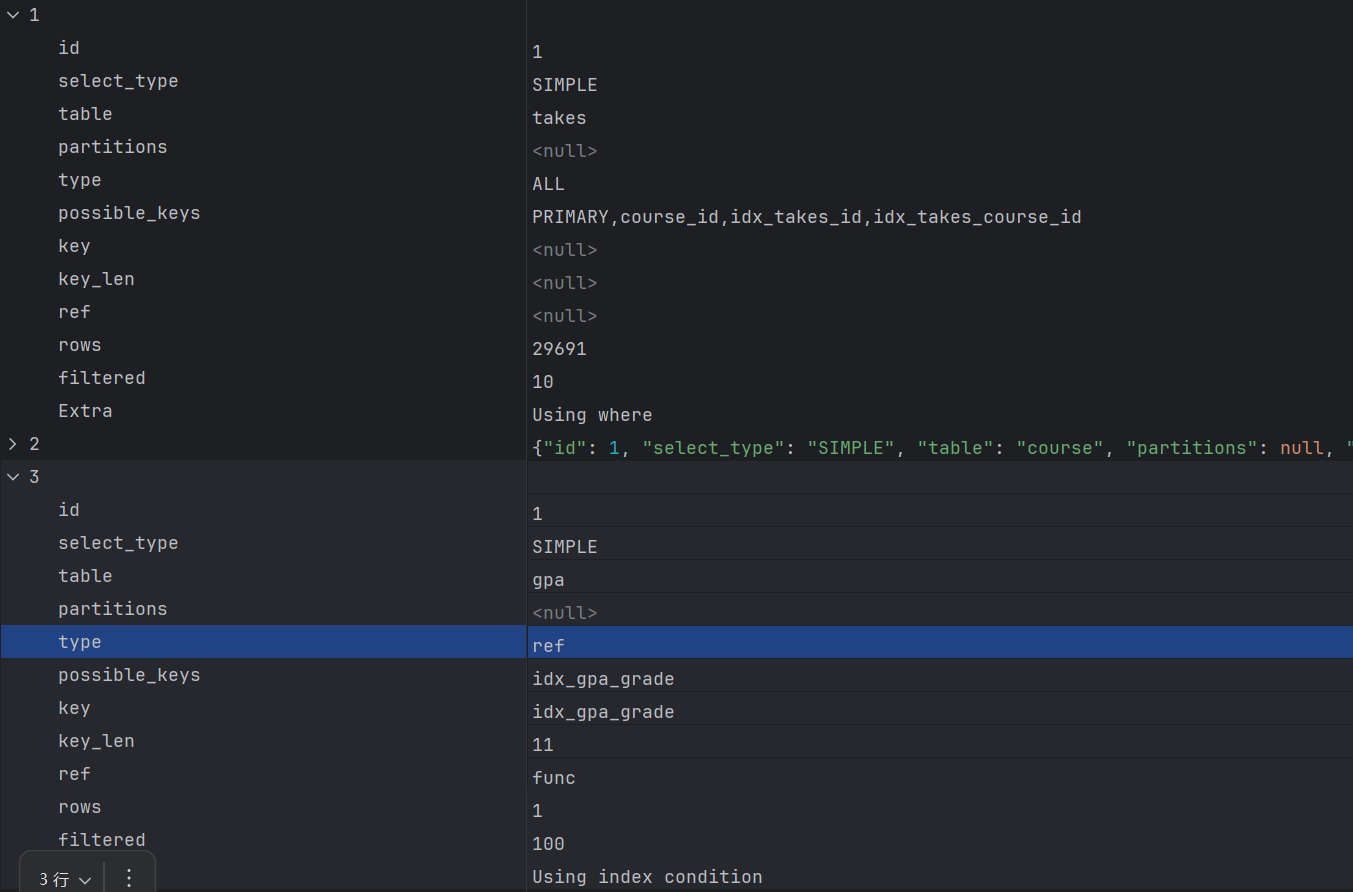
\includegraphics[width=\textwidth]{./images/15.EXPLAIN-4.png}
			\caption{第四个语句的EXPLAIN结果}
		\end{minipage}
	\end{figure}
	
	结合我在\mybox[blue]{3.2章节内的表1和表2}中提到的内容,我们需要对于type=ALL的语句进行更新。
	
	可以通过添加索引来优化查询性能,尤其是在我的查询逻辑中,有部分性能瓶颈正是因为没有使用索引或者索引失效。
	
	\subsubsection{更新第一条SQL语句}
	
	由图12可以看到,第一条SQL语句查询的执行计划中,对student表进行了\textbf{全表扫描},没有使用索引,导致查询性能较差。可以通过为student表的相关字段创建索引来优化查询性能。
	
	再来看一下第一条SQL语句的\textbf{EXPLAIN ANALYZE}的结果:
	
	\begin{figure}[H]
		\centering
		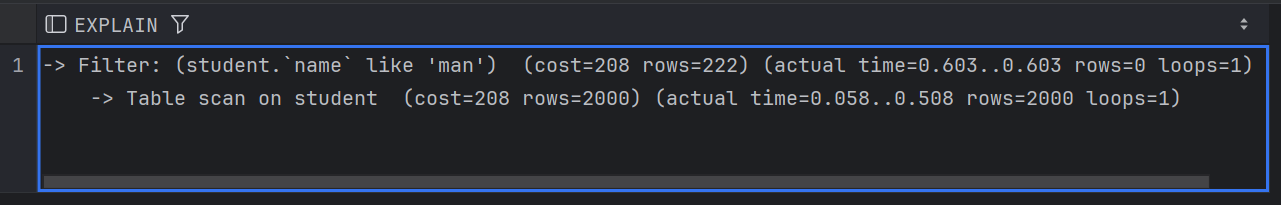
\includegraphics[width=15cm]{./images/16.EXPLAIN_ANALYZE-1.png}
		\caption{EXPLAIN\_ANALYZE第一条SQL语句}
	\end{figure}
	
	从cost上看,student表的扫描成本较高,因此应优化student表的查询性能。
	
	原始的查询语句:
	
	\begin{lstlisting}[language=sql, title=原始的子串查询, tabsize=4]
		SELECT ID, name, dept_name, tot_cred 
		FROM student 
		WHERE name LIKE '%子串%';
	\end{lstlisting}
	
	其过程可以用下图来解释:
	
	\begin{center}
		\begin{tikzpicture}[
			node distance=1cm and 0.5cm,
			every node/.style={draw, rectangle, align=center, minimum width=3cm},
			operation/.style={ellipse, draw, align=center},
			arrow/.style={-Stealth, thick, shorten <=2mm, shorten >=2mm}
			]
			
			% Nodes
			\node (start) [operation] {开始};
			\node (scan) [below=of start] {表扫描 student};
			\node (filter) [below=of scan] {过滤: name LIKE ('\%子串\%')};
			\node (project) [below=of filter] {投影: ID, name, dept\_name, tot\_cred};
			\node (end) [operation, below=of project] {结束};
			
			% Connections
			\draw [arrow] (start) -- (scan);
			\draw [arrow] (scan) -- (filter);
			\draw [arrow] (filter) -- (project);
			\draw [arrow] (project) -- (end);
			
		\end{tikzpicture}
	\end{center}
	
	\mybox[red]{问题:}
	
	\begin{enumerate}[label=\textbullet]
		\item \% 开头的 LIKE 查询无法使用普通索引,会导致全表扫描。
	\end{enumerate}
	
	\mybox[red]{优化方案:}
	
	\begin{enumerate}[label=\textbullet]
		\item 此处我的思路是在 student 表的 name 列上创建一个全文索引(FULLTEXT)(针对模糊查询),用于优化对该列中文本数据的搜索查询。
	\end{enumerate}
	
	\mybox[red]{代码如下:}
	
	\begin{lstlisting}[language=sql, title=student.name 上添加 全文索引(FULLTEXT)(针对模糊查询), tabsize=4]
		ALTER TABLE student ADD FULLTEXT(name);
	\end{lstlisting}
	
	然后查询改为:
	
	\begin{lstlisting}[language=sql, title=更新后的查询语句, tabsize=4]
		SELECT ID, name, dept_name, tot_cred 
		FROM student 
		WHERE MATCH(name) AGAINST ('子串');
	\end{lstlisting}
	
	其过程可以用下图来解释:
	
	\begin{center}
		\begin{tikzpicture}[
			node distance=1cm and 0.5cm,
			every node/.style={draw, rectangle, rounded corners, align=center, minimum width=4cm},
			operation/.style={ellipse, draw, align=center},
			arrow/.style={-Stealth, thick, shorten <=2mm, shorten >=2mm}
			]
			
			% Nodes
			\node (start) [operation] {开始};
			\node (fulltext_index) [below=of start] {为 student.name 添加 FULLTEXT 索引};
			\node (select) [below=of fulltext_index] {执行 SELECT 查询};
			\node (match) [below=of select] {全文匹配: MATCH(name) AGAINST ('子串')};
			\node (project) [below=of match] {投影: ID, name, dept\_name, tot\_cred};
			\node (end) [operation, below=of project] {结束};
			
			% Connections
			\draw [arrow] (start) -- (fulltext_index);
			\draw [arrow] (fulltext_index) -- (select);
			\draw [arrow] (select) -- (match);
			\draw [arrow] (match) -- (project);
			\draw [arrow] (project) -- (end);
			
		\end{tikzpicture}
	\end{center}
	
	\mybox[red]{更新结果}
	
	重新对于上述sql语句进行\textbf{EXPLAIN}解释,得到的结果如下图所示:
	
	\begin{figure}[H]
		\centering
		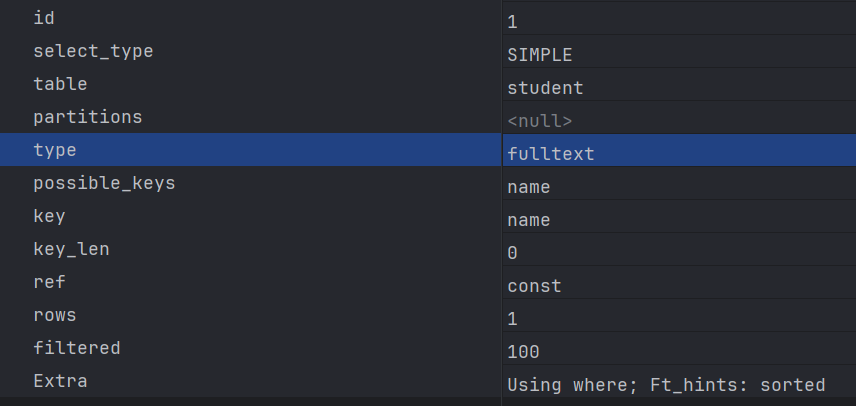
\includegraphics[width=11cm]{./images/17.更新结果-1-1.png}
		\caption{第一条sql语句更新结果 - EXPLAIN}
	\end{figure}
	
	再来用EXPLAIN ANALYZE来检查一下:
	
	\begin{figure}[H]
		\centering
		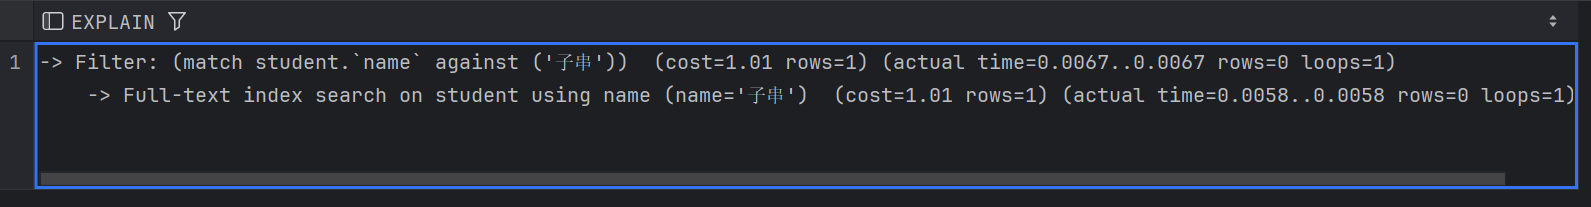
\includegraphics[width=15cm]{./images/18.更新结果-1-2.png}
		\caption{第一条sql语句更新结果 - EXPLAIN ANALYZE}
	\end{figure}
	
	这里我们看到type变为了fulltext,const值也从208减少为了1.01,大幅减少,优化成功。
	
	\subsubsection{更新第二条SQL语句}
	
	由图13可以看到,第二条SQL语句查询的执行计划中,对student表进行了\textbf{全表扫描},没有使用索引,导致查询性能较差。可以通过为student表的相关字段创建索引来优化查询性能。
	
	再来看一下第二条SQL语句的\textbf{EXPLAIN ANALYZE}的结果:
	
	\begin{figure}[H]
		\centering
		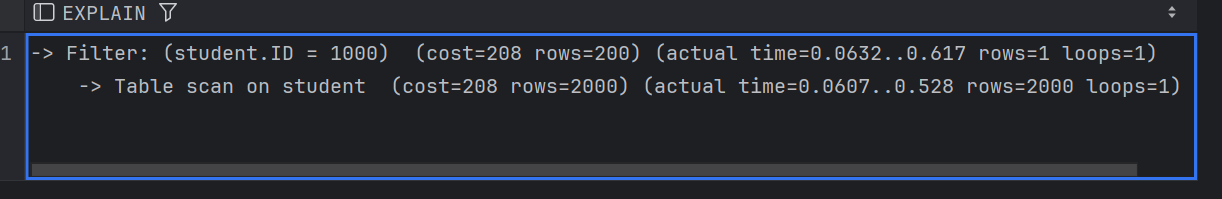
\includegraphics[width=15cm]{./images/19.EXPLAIN_ANALYZE-2.png}
		\caption{EXPLAIN\_ANALYZE第二条SQL语句}
	\end{figure}
	
	从cost上看,student表的扫描成本较高,因此应优化student表的查询性能。
	
	原始的查询语句:
	
	\begin{lstlisting}[language=sql, title=原始的子串查询, tabsize=4]
		SELECT ID, name, dept_name, tot_cred
		FROM student
		WHERE ID = ?;
	\end{lstlisting}
	
	其过程可以用下图来解释:
	
	\begin{center}
		\begin{tikzpicture}[
			node distance=1.5cm and 0.5cm,
			every node/.style={draw, rectangle, rounded corners, align=center, minimum width=4cm},
			operation/.style={ellipse, draw, align=center},
			arrow/.style={-Stealth, thick, shorten <=2mm, shorten >=2mm}
			]
			
			% Nodes
			\node (start) [operation] {开始};
			\node (param_query) [below=of start] {执行参数化查询};
			\node (index_lookup) [below=of param_query] {索引查找: 使用 ID 索引};
			\node (project) [below=of index_lookup] {投影: ID, name, dept\_name, tot\_cred};
			\node (end) [operation, below=of project] {结束};
			
			% Connections
			\draw [arrow] (start) -- (param_query);
			\draw [arrow] (param_query) -- (index_lookup);
			\draw [arrow] (index_lookup) -- (project);
			\draw [arrow] (project) -- (end);
			
		\end{tikzpicture}
	\end{center}
	
	\mybox[red]{问题:}
	
	\begin{enumerate}[label=\textbullet]
		\item 该查询语句虽然使用主键进行筛选,但由于数据库未正确使用索引(可能是索引未生效或统计信息不准确),导致对 student 表进行了全表扫描,从而降低了查询效率。
	\end{enumerate}
	
	\mybox[red]{优化方案:}
	
	\begin{enumerate}[label=\textbullet]
		\item 此处我的思路是如果 student 表中的 ID 字段尚未设为主键,应显式地为其创建索引,以便查询时可利用索引进行快速定位。
	\end{enumerate}
	
	\mybox[red]{代码如下:}
	
	\begin{lstlisting}[language=sql, title=student.id 上显式地为其创建索引, tabsize=4]
		CREATE INDEX idx_takes_id ON takes (ID);
	\end{lstlisting}
	
	然后查询改为:
	
	\begin{lstlisting}[language=sql, title=更新后的查询语句, tabsize=4]
		SELECT ID, name, dept_name, tot_cred
		FROM student FORCE INDEX (idx_student_id)
		WHERE ID = 1000;
	\end{lstlisting}
	
	其过程可以用下图来解释:
	
	\begin{center}
		\begin{tikzpicture}[
			node distance=1.5cm and 0.5cm,
			every node/.style={draw, rectangle, rounded corners, align=center, minimum width=4cm},
			operation/.style={ellipse, draw, align=center},
			arrow/.style={-Stealth, thick, shorten <=2mm, shorten >=2mm}
			]
			
			% Nodes
			\node (start) [operation] {开始};
			\node (create_index) [below=of start] {创建索引 idx\_student\_id};
			\node (select) [below=of create_index] {执行 SELECT 查询};
			\node (force_index) [below=of select] {强制使用索引 idx\_student\_id};
			\node (index_lookup) [below=of force_index] {索引查找: ID = 1000};
			\node (project) [below=of index_lookup] {投影: ID, name, dept\_name, tot\_cred};
			\node (end) [operation, below=of project] {结束};
			
			% Connections
			\draw [arrow] (start) -- (create_index);
			\draw [arrow] (create_index) -- (select);
			\draw [arrow] (select) -- (force_index);
			\draw [arrow] (force_index) -- (index_lookup);
			\draw [arrow] (index_lookup) -- (project);
			\draw [arrow] (project) -- (end);
			
		\end{tikzpicture}
	\end{center}
	
	\mybox[red]{更新结果}
	
	重新对于上述sql语句进行\textbf{EXPLAIN ANALYZE}解释,得到的结果如下图所示:
	
	\begin{figure}[H]
		\centering
		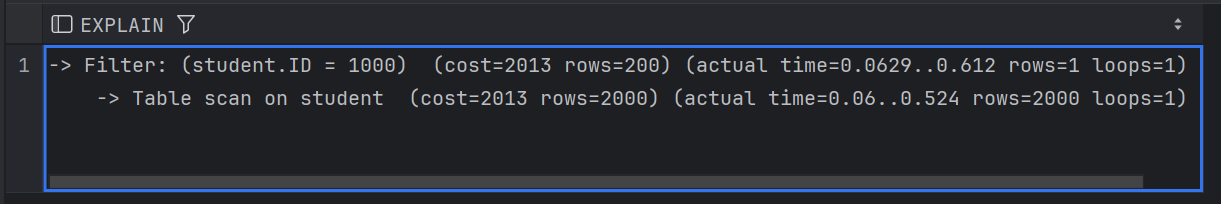
\includegraphics[width=15cm]{./images/20.更新结果-2.png}
		\caption{第二条sql语句更新结果 - EXPLAIN ANALYZE}
	\end{figure}
	
	优化后的 SQL 查询将能够利用索引,减少对整个 student 表的扫描,从而提高查询效率。通过再次执行 EXPLAIN 或 EXPLAIN ANALYZE,可以观察到执行计划的 \texttt{type} 字段从 \texttt{ALL} 变为 \texttt{ref},cost 也会明显降低,验证了优化效果。
	
	\subsubsection{更新第三条SQL语句}
	
	由图14可以看到,第三条SQL语句查询的执行计划中,对takes表进行了\textbf{全表扫描},没有使用索引,导致查询性能较差;而对于course表进行的是\textbf{eq\_ref}。可以通过为takes表的相关字段创建索引来优化查询性能。
	
	再来看一下第三条SQL语句的\textbf{EXPLAIN ANALYZE}的结果:
	
	\begin{figure}[H]
		\centering
		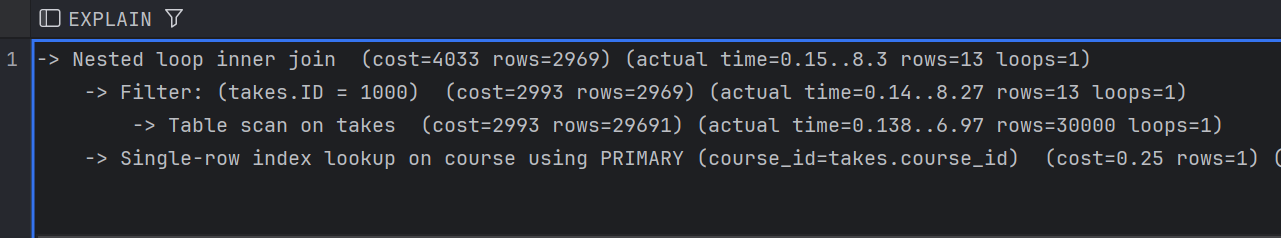
\includegraphics[width=15cm]{./images/21.EXPLAIN_ANALYZE-3.png}
		\caption{EXPLAIN\_ANALYZE第三条SQL语句}
	\end{figure}
	
	从cost上看,takes表的扫描成本较高,而course表的扫描的成本很小,因此应优化takes表的查询性能。
	
	原始的查询语句:
	
	\begin{lstlisting}[language=sql, title=原始的子串查询, tabsize=4]
		SELECT takes.course_id, year, semester, title, dept_name, grade, credits
		FROM takes
				JOIN course ON takes.course_id = course.course_id
		WHERE ID = ?;
	\end{lstlisting}
	
	其过程可以用下图来解释:
	
	\begin{center}
		\begin{tikzpicture}[
			node distance=1.5cm and 0.5cm,
			every node/.style={draw, rectangle, rounded corners, align=center, minimum width=4cm},
			operation/.style={ellipse, draw, align=center},
			arrow/.style={-Stealth, thick, shorten <=2mm, shorten >=2mm}
			]
			
			% Nodes
			\node (start) [operation] {开始};
			\node (param_query) [below=of start] {执行参数化查询};
			\node (join) [below=of param_query] {连接 takes 和 course 表};
			\node (index_lookup) [below=of join] {索引查找: ID = ?};
			\node (filter) [below=of index_lookup] {过滤: takes.course\_id = course.course\_id};
			\node (project) [below=of filter] {投影: course\_id, year, semester, title, dept\_name, grade, credits};
			\node (end) [operation, below=of project] {结束};
			
			% Connections
			\draw [arrow] (start) -- (param_query);
			\draw [arrow] (param_query) -- (join);
			\draw [arrow] (join) -- (index_lookup);
			\draw [arrow] (index_lookup) -- (filter);
			\draw [arrow] (filter) -- (project);
			\draw [arrow] (project) -- (end);
			
		\end{tikzpicture}
	\end{center}
	
	\mybox[red]{问题:}
	
	\begin{enumerate}[label=\textbullet]
		\item 如图所示,takes 表在该查询中进行了 \textbf{全表扫描(type = ALL)},说明 MySQL 没有使用索引来定位指定学生的课程信息。
		
		\item 根据 EXPLAIN ANALYZE 的输出,其成本远高于 course 表的处理成本,主要开销集中在 takes 表上。因此,应重点优化 takes 表的查询效率。
	\end{enumerate}
	
	\mybox[red]{优化方案:}
	
	\begin{enumerate}[label=\textbullet]
		\item 此处我的思路是为 takes 表的 ID 和 course\_id 字段创建索引:原始语句中通过 \texttt{WHERE ID = ?} 条件筛选学生,因此为 \texttt{takes.ID} 添加索引可以显著提高定位速度。
		
	\end{enumerate}
	
	\clearpage
	
	\mybox[red]{代码如下:}
	
	\begin{lstlisting}[language=sql, title=student.name 上添加 全文索引(FULLTEXT)(针对模糊查询), tabsize=4]
		CREATE INDEX idx_takes_id ON takes (ID);
		CREATE INDEX idx_takes_course_id ON takes (course_id);
	\end{lstlisting}
	
	然后查询改为:
	
	\begin{lstlisting}[language=sql, title=更新后的查询语句, tabsize=4]
		SELECT takes.course_id,
			   year,
			   semester,
			   title,
			   dept_name,
			   grade,
			   credits
		FROM takes
				JOIN course ON takes.course_id = course.course_id
		WHERE takes.ID = ?;
	\end{lstlisting}
	
	其过程可以用下图来解释:
	
	
	\begin{center}
		\begin{tikzpicture}[
			node distance=1.5cm and 0.5cm,
			every node/.style={draw, rectangle, rounded corners, align=center, minimum width=4cm},
			operation/.style={ellipse, draw, align=center},
			arrow/.style={-Stealth, thick, shorten <=2mm, shorten >=2mm}
			]
			
			% Nodes
			\node (start) [operation] {开始};
			\node (create_index1) [below=of start] {为 takes.ID 创建索引 idx\_takes\_id};
			\node (create_index2) [below=of create_index1] {为 takes.course\_id 创建索引 idx\_takes\_course\_id};
			\node (select) [below=of create_index2] {执行 SELECT 查询};
			\node (index_lookup) [below=of select] {索引查找: takes.ID = ?};
			\node (join) [right=of index_lookup, xshift=4cm] {连接 takes 和 course 表};
			\node (filter) [above=of join] {过滤: takes.course\_id = course.course\_id};
			\node (project) [above=of filter] {投影: course\_id, year, semester,\\ title, dept\_name, grade, credits};
			\node (end) [operation, above=of project] {结束};
			
			% Connections
			\draw [arrow] (start) -- (create_index1);
			\draw [arrow] (create_index1) -- (create_index2);
			\draw [arrow] (create_index2) -- (select);
			\draw [arrow] (select) -- (index_lookup);
			\draw [arrow] (index_lookup) -- (join);
			\draw [arrow] (join) -- (filter);
			\draw [arrow] (filter) -- (project);
			\draw [arrow] (project) -- (end);
			
		\end{tikzpicture}
	\end{center}
	
	\mybox[red]{更新结果}
	
	重新对于上述sql语句进行\textbf{EXPLAIN ANALYZE}解释,得到的结果如下图所示:
	
	\begin{figure}[H]
		\centering
		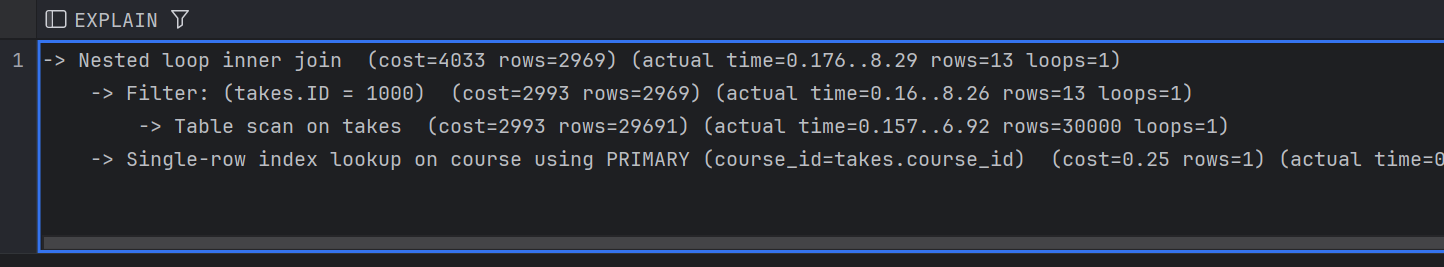
\includegraphics[width=15cm]{./images/22.更新结果-3.png}
		\caption{第三条sql语句更新结果 - EXPLAIN ANALYZE}
	\end{figure}
	
	可以观察到 takes 表的 rows 数量显著减少,查询成本更低,优化完成。
	
	\subsubsection{更新第四条SQL语句}
	
	由图15可以看到,第四条SQL语句查询的执行计划中,对takes表进行了\textbf{全表扫描},没有使用索引,导致查询性能较差;而对于course表进行的是\textbf{eq\_ref},对于gpa表进行的是\textbf{ref}。可以通过为takes表的相关字段创建索引来优化查询性能。
	
	再来看一下第三条SQL语句的\textbf{EXPLAIN ANALYZE}的结果:
	
	\begin{figure}[H]
		\centering
		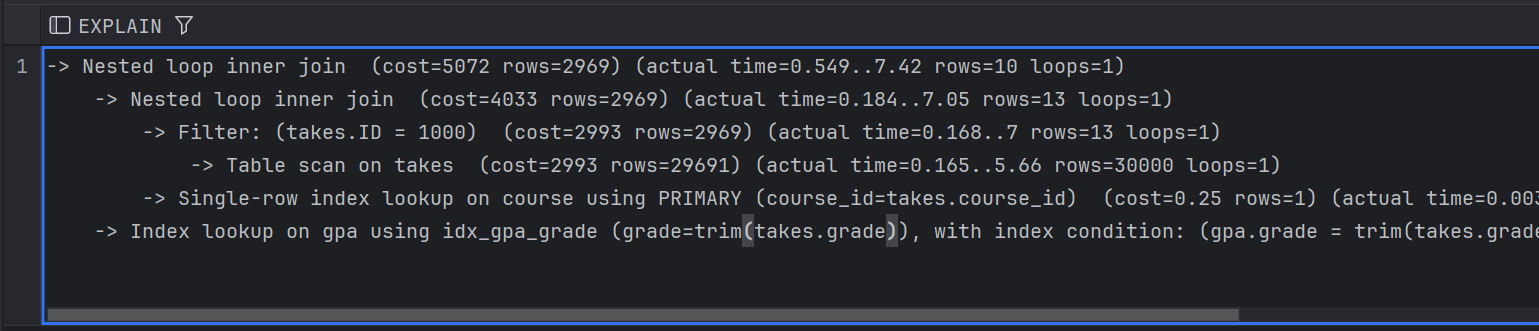
\includegraphics[width=15cm]{./images/23.EXPLAIN_ANALYZE-4.png}
		\caption{EXPLAIN\_ANALYZE第四条SQL语句}
	\end{figure}
	
	从cost上看,takes表的扫描成本较高,而course表和gpa表的扫描的成本很小,因此应优化takes表的查询性能。
	
	原始的查询语句:
	
	\begin{lstlisting}[language=sql, title=原始的子串查询, tabsize=4]
		SELECT grade_point, credits
		FROM (takes JOIN course ON takes.course_id = course.course_id)
				JOIN gpa ON gpa.grade = TRIM(takes.grade)
		WHERE ID = ?;
	\end{lstlisting}
	
	其过程可以用下图来解释:
	
	
	\begin{center}
		\begin{tikzpicture}[
			node distance=1.5cm and 0.5cm,
			every node/.style={draw, rectangle, rounded corners, align=center, minimum width=4cm},
			operation/.style={ellipse, draw, align=center},
			arrow/.style={-Stealth, thick, shorten <=2mm, shorten >=2mm}
			]
			
			% Nodes
			\node (start) [operation] {开始};
			\node (param_query) [below=of start] {执行参数化查询};
			\node (join1) [below=of param_query] {连接 takes 和 course 表};
			\node (join2) [below=of join1] {连接结果与 gpa 表};
			\node (trim) [below=of join2] {TRIM(takes.grade) 转换};
			\node (filter) [right=of trim, xshift=3cm] {过滤: gpa.grade = takes.grade};
			\node (index_lookup) [above=of filter] {索引查找: takes.ID = ?};
			\node (project) [above=of index_lookup] {投影: grade\_point, credits};
			\node (end) [operation, above=of project] {结束};
			
			% Connections
			\draw [arrow] (start) -- (param_query);
			\draw [arrow] (param_query) -- (join1);
			\draw [arrow] (join1) -- (join2);
			\draw [arrow] (join2) -- (trim);
			\draw [arrow] (trim) -- (filter);
			\draw [arrow] (filter) -- (index_lookup);
			\draw [arrow] (index_lookup) -- (project);
			\draw [arrow] (project) -- (end);
			
		\end{tikzpicture}
	\end{center}
	
	\mybox[red]{问题:}
	
	\begin{enumerate}[label=\textbullet]
		\item 如图所示,takes 表在该查询中依然进行了 \textbf{全表扫描(type = ALL)},说明针对 \texttt{ID} 的筛选条件未能使用索引,导致整体查询性能较低。
		
		\item 从 EXPLAIN ANALYZE 的结果来看,takes 表的扫描成本显著高于其他两个表,因此优化应优先聚焦于 takes 表。
		
	\end{enumerate}
	
	\mybox[red]{优化方案:}
	
	\begin{enumerate}[label=\textbullet]
		\item 此处我的思路与问题三一致,是为 takes 表的 ID 和 course\_id 字段创建索引:原始语句中通过 \texttt{WHERE ID = ?} 条件筛选学生,因此为 \texttt{takes.ID} 添加索引可以显著提高定位速度。
		
		\item 并添加 gpa.grade 的索引
	\end{enumerate}
	
	\mybox[red]{代码如下:}
	
	\begin{lstlisting}[language=sql, title=student.name 上添加 全文索引(FULLTEXT)(针对模糊查询), tabsize=4]
		CREATE INDEX idx_takes_id ON takes(ID);
	\end{lstlisting}
	
	然后查询改为:
	
	\begin{lstlisting}[language=sql, title=更新后的查询语句, tabsize=4]
		SELECT grade_point, credits
		FROM takes
				JOIN course ON takes.course_id = course.course_id
				JOIN gpa ON gpa.grade = takes.grade -- 去掉 TRIM()
		WHERE takes.ID = 1000;
	\end{lstlisting}
	
	其过程可以用下图来解释:
	
	\begin{center}
		\begin{tikzpicture}[
			node distance=1.5cm and 0.5cm,
			every node/.style={draw, rectangle, rounded corners, align=center, minimum width=4cm},
			operation/.style={ellipse, draw, align=center},
			arrow/.style={-Stealth, thick, shorten <=2mm, shorten >=2mm}
			]
			
			% Nodes
			\node (start) [operation] {开始};
			\node (index_creation) [below=of start] {为 takes.ID 创建索引 idx\_takes\_id};
			\node (select) [below=of index_creation] {执行 SELECT 查询};
			\node (index_lookup) [below=of select] {索引查找: takes.ID = 1000};
			\node (join1) [below=of index_lookup] {连接 takes 和 course 表};
			\node (join2) [right=of join1, xshift=3cm] {连接结果与 gpa 表};
			\node (filter) [above=of join2] {过滤: gpa.grade = takes.grade};
			\node (project) [above=of filter] {投影: grade\_point, credits};
			\node (end) [operation, above=of project] {结束};
			
			% Connections
			\draw [arrow] (start) -- (index_creation);
			\draw [arrow] (index_creation) -- (select);
			\draw [arrow] (select) -- (index_lookup);
			\draw [arrow] (index_lookup) -- (join1);
			\draw [arrow] (join1) -- (join2);
			\draw [arrow] (join2) -- (filter);
			\draw [arrow] (filter) -- (project);
			\draw [arrow] (project) -- (end);
			
		\end{tikzpicture}
	\end{center}
	
	\mybox[red]{更新结果}
	
	重新对于上述sql语句进行\textbf{EXPLAIN ANALYZE}解释,得到的结果如下图所示:
	
	\begin{figure}[H]
		\centering
		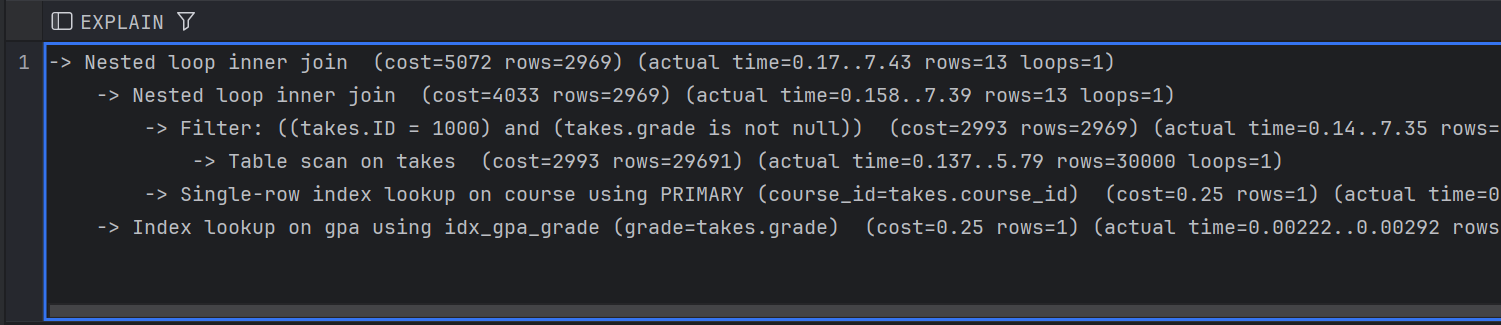
\includegraphics[width=15cm]{./images/24.更新结果-4.png}
		\caption{第四条sql语句更新结果 - EXPLAIN ANALYZE}
	\end{figure}
	
	可以观察到 takes 表的 rows 数量显著减少,查询成本更低,优化完成。
	
	至此,实验已经基本完成,接下来是我本次实验中遇到的问题和实验小结。
	
	\section{存在的问题及解决方案}
	
	在数据库查询优化的学习过程中,我遇到了几个关键的挑战,并找到了相应的解决方案:
	
	\subsection{存在的问题:}
	
	\begin{enumerate}[noitemsep, label={{\arabic*})}]
		\item 对于如何有效解读 \texttt{EXPLAIN} 和 \texttt{EXPLAIN ANALYZE} 的输出结果感到困惑。
		\item 遇到了PostgreSQL和MySQL在查询计划输出格式上的差异问题。
	\end{enumerate}\textbf{}
	
	\subsection{解决方案:}
	
	\begin{enumerate}[noitemsep, label={{\arabic*})}]
		\item 我通过在线教程和专业论坛,学习了如何解读这些工具的输出结果,并了解了如何利用这些信息来优化数据库查询的性能。
		\item 我查阅了PostgreSQL的官方文档,了解了其查询计划的详细格式,并学会了如何分析这些信息以优化查询。
	\end{enumerate}\textbf{}
	
	\section{实验小结}
	
	通过这次实验,我不仅学会了如何使用 \texttt{EXPLAIN} 和 \texttt{EXPLAIN ANALYZE} 来分析数据库查询的执行计划,还学会了如何根据这些信息来优化查询性能。此外,我还通过实际应用这些工具来分析课程项目中的查询,进一步加深了对查询执行计划的理解。这次实验让我对数据库查询优化有了更深刻的认识,并激发了我进一步探索这一领域的兴趣。
	
\end{document}
